% ALGUNOS PAQUETES REQUERIDOS (EN UBUNTU): %
% ========================================
% %
% texlive-latex-base %
% texlive-latex-recommended %
% texlive-fonts-recommended %
% texlive-latex-extra %
% texlive-lang-spanish (en ubuntu 13.10) %
% ******************************************************** %

\documentclass[a4paper]{article}
\usepackage[spanish]{babel}
\usepackage[utf8]{inputenc}
\usepackage{fancyhdr}
\usepackage[pdftex]{graphicx}
\usepackage{sidecap}
\usepackage{caption}
\usepackage{subcaption}
\usepackage{booktabs}
\usepackage{makeidx}
\usepackage{float}
\usepackage{amsmath, amsthm, amssymb}
\usepackage{amsfonts}
\usepackage{sectsty}
\usepackage{wrapfig}
\usepackage{listings}
\usepackage{enumitem}
\usepackage{hyperref}
\usepackage{listings}
\usepackage{listingsutf8}
\usepackage{enumitem}

% Para ver los marcos
% \usepackage{showframe}

\newcommand{\ord}{\ensuremath{\operatorname{O}}}
\newcommand{\nat}{\ensuremath{\mathbb{N}}}
\renewcommand{\thesubsubsection}{\thesubsection.\alph{subsubsection}}

% Lemas, definiciones, etc.
\theoremstyle{remark}
\newtheorem*{obs}{Observación}
\newtheorem*{nota}{Notación}
\newtheorem*{cor}{Corolario}
\theoremstyle{definition}
\newtheorem*{defi}{Definición}
\theoremstyle{plain}
\newtheorem{teo}{Teorema}
\newtheorem{lema}{Lema}
\newtheorem{prop}{Propiedad}

\usepackage{fancyhdr}
% \pagestyle{fancy}
%\renewcommand{\chaptermark}[1]{\markboth{#1}{}}
\renewcommand{\sectionmark}[1]{\markright{\thesection\ - #1}}
\fancyhf{}
% \fancyhead[LO]{Sección \rightmark} % \thesection\

% \fancyfoot[RO]{\thepage}
\renewcommand{\headrulewidth}{0.5pt}
\renewcommand{\footrulewidth}{0.5pt}
%\setlength{\hoffset}{-0.8in}
\setlength{\textwidth}{16cm}
\setlength{\hoffset}{-1.1cm}
\setlength{\headsep}{0.5cm}
\setlength{\textheight}{25cm}
\setlength{\voffset}{-0.7in}
\setlength{\headwidth}{\textwidth}
\setlength{\headheight}{13.1pt}
\renewcommand{\baselinestretch}{1.1} % line spacing


\begin{document}

\title{Teoría de las comunicaciones}
\author{Manuel Mena}
\maketitle

\tableofcontents

\newpage
\section{Práctica 1}

\subsection{}

\subsubsection{}
$I(s) = -log_2(P(s))$

\begin{tabular}{rl}
$H(S)$ & $= \sum_{s \in S}(P(s) I(s))$ \\
& $= (P(s_0) I(s_0)) + (P(s_1) I(s_1))$ \\
& $= (p_0 (-log_2(p_0))) + (1 - p_0) (-log_2(1 - p_0)))$ \\
& $= -p_0 log_2(p_0) - log_2(1 - p_0) + p_0 log_2(1 - p_0)$ \\
& $= p_0(log_2(1 - p_0) -log_2(p_0)) - log_2(1 - p_0)$ \\
& $= p_0 * log_2(\frac{1 - p_0}{p_0}) - log_2(1 - p_0)$ \\
\end{tabular}

\subsubsection{}

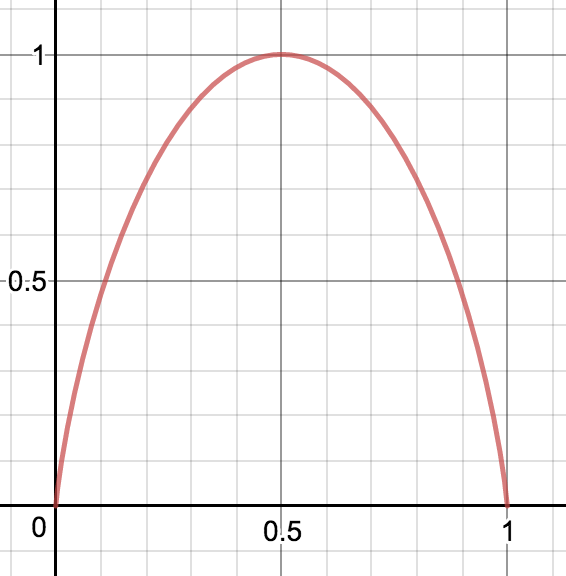
\includegraphics{imagenes/1_1_b.png}

\subsection{}

\subsubsection{}
El tercero

\subsubsection{}
El segundo y el tercero

\subsubsection{}
\begin{tabular}{rl}
$H(S)$ & $= \sum_{s \in S}(P(s) I(s))$ \\
& $= 0.4 (-log_2(0.4)) + 0.3 (-log_2(0.3)) + 0.2 (-log_2(0.2)) + 0.1 (-log_2(0.1))$ \\
& $= 1.84643934467$ \\
\end{tabular}

\begin{tabular}{rl}
$L(segundo)$ & $= \sum_{s \in S}(P(s)|C(s)|)$ \\
& $= 0.4 * 1 + 0.3 * 2 + 0.2 * 3 + 0.1 * 3$ \\
& $= 1.9$ \\
\end{tabular}

\begin{tabular}{rl}
$L(tercero)$ & $= \sum_{s \in S}(P(s)|C(s)|)$ \\
& $= 0.4 * 1 + 0.3 * 2 + 0.2 * 3 + 0.1 * 4$ \\
& $= 2$ \\
\end{tabular}

Eficiencia segundo: 0,9718101814

Eficiencia tercero: 0,9232196723

El segundo es más eficiente.

\subsubsection{}
No, puesto que $H(S) \leq L(C)$ en ambos casos.

\subsection{}

\subsubsection{}
\begin{tabular}{rl}
$H(S)$ & $= \sum_{s \in S}(P(s) I(s))$ \\
& $= 0.5 (-log_2(0.5)) + 0.5 (-log_2(0.5))$ \\
& $= 1$ \\
\end{tabular}

\begin{tabular}{rl}
$L(C)$ & $= \sum_{s \in S}(P(s) |C(s)|)$ \\
& $= 0.5 * 1 + 0.5 * 1$ \\
& $= 1$ \\
\end{tabular}

\subsubsection{}
\begin{tabular}{rl}
$H(S)$ & $= \sum_{s \in S}(P(s) I(s))$ \\
& $= 0.25 (-log_2(0.25)) + 0.25 (-log_2(0.25)) + 0.25 (-log_2(0.25)) + 0.25 (-log_2(0.25))$ \\
& $= 2$ \\
\end{tabular}

\begin{tabular}{rl}
$L(C)$ & $= \sum_{s \in S}(P(s) |C(s)|)$ \\
& $= 0.25 * 2 + 0.25 * 2 + 0.25 * 2 + 0.25 * 2$ \\
& $= 2$ \\
\end{tabular}

\subsubsection{}
\begin{tabular}{rl}
$H(S)$ & $= \sum_{s \in S}(P(s) I(s))$ \\
& $= \frac{1}{6} (-log_2(\frac{1}{6})) + \frac{1}{6} (-log_2(\frac{1}{6})) + \frac{1}{6} (-log_2(\frac{1}{6})) + \frac{1}{6} (-log_2(\frac{1}{6})) + \frac{1}{6} (-log_2(\frac{1}{6})) + \frac{1}{6} (-log_2(\frac{1}{6}))$ \\
& $= 2.58496250072$ \\
\end{tabular}

\begin{tabular}{rl}
$L(C)$ & $= \sum_{s \in S}(P(s) |C(s)|)$ \\
& $= \frac{1}{6} (-log_2(\frac{1}{6})) + \frac{1}{6} (-log_2(\frac{1}{6})) + \frac{1}{6} (-log_2(\frac{1}{6})) + \frac{1}{6} (-log_2(\frac{1}{6})) + \frac{1}{6} (-log_2(\frac{1}{6})) + \frac{1}{6} (-log_2(\frac{1}{6}))$ \\
& $= 2.58496250072$ \\
\end{tabular}

\subsubsection{}
\begin{tabular}{rl}
$H(S)$ & $= \sum_{s \in S}(P(s) I(s))$ \\
& $= 0.125 (-log_2(0.125)) * 8$ \\
& $= 3$ \\
\end{tabular}

\subsubsection{}
\begin{tabular}{rl}
$H(S)$ & $= \sum_{s \in S}(P(s) I(s))$ \\
& $= 0.1 (-log_2(0.1)) * 10$ \\
& $= -log_2(0.1)$ \\
& $= log_2(10)$ \\
& $= 3.32192809489$ \\
\end{tabular}

\subsubsection{}
\begin{tabular}{rl}
$H(S)$ & $= \sum_{s \in S}(P(s) I(s))$ \\
& $= \frac{1}{n} (-log_2(\frac{1}{n})) * n$ \\
& $= -log_2(\frac{1}{n})$ \\
& $= log_2(n)$ \\
\end{tabular}

\subsection{}
Acá lo mas importante es notar que cada vez que la fuente $D$ toma un símbolo
es independiente de la anterior, entonces se puede definir
$P_D(s) = (P_D(A) * P_A(s) si s \in A sino P_D(B) * P_B(s))$, con $P_D(A)$ y
$P_D(B)$ la probabilidad de que $D$ saque un símbolo de $A$ y de $B$,
respectivamente. Entonces la solución sería:

\begin{enumerate}
\item $P_D(s) = 1/16$ si $s \in A$ sino $1/32$, no es equiprobable
\item $P_D(s) = 1/64$ si $s \in A$ sino $3/64$, no es equiprobable
\item $P_D(s) = 1/32$ si $s \in A$ sino $3/64$, no es equiprobable
\item $P_D(s) = 1/12$ si $s \in A$ sino $1/48$, no es equiprobable
\end{enumerate}

\subsection{}

\subsubsection{}
Como la fuente es equiprobable:

\begin{tabular}{rl}
$H(S) $ & $= log_2|S|$ \\
&$= log_2(10^{640*480})$ \\
&$= 640 * 480 * log_2(10)$ \\
\end{tabular}

\subsubsection{}
En esta fuente equiprobable, tenemos que $H(S) = log_2(n)$, no siendo $n$ una potencia de 2. Esto implica que no podemos pensar en recurrir a un código (óptimo) que asigne $log_2(n)$ bits por imagen, pues por supuesto estos valores deben ser números enteros. No obstante, la aproximación más cercana a este valor es tomar exactamente $\lceil log_2(n) \rceil$ bits por imagen. De esta forma podremos armar un código que sea unívocamente decodificable (cada imagen recibe una tira de bits distinta) y localmente óptimo, entendiendo por esto que todo otro código que mapee cada imagen a una tira de bits de igual largo debe necesariamente poseer una longitud media igual o mayor.
Como nota adicional, extrapolando los conceptos plasmados en la resolución de este ejercicio, es interesante pensar en si, efectivamente, dada una fuente equiprobable S' de m símbolos, y dado un código C que actúe sobre S' definiendo para cada símbolo una codificación de largo $\lceil log_2(m) \rceil$ bits, se tiene que C es óptimo. Cuando m es potencia de 2, la respuesta es afirmativa (¿por qué?). En cualquier otro caso, y quizás yendo a contramano de la intuición, la respuesta es que no. Como ejemplo sencillo, considerar el caso en el que $m = 3$. Como $\lceil log_2(m) \rceil = 2$, tenemos que $L(C) = 2$. Sin embargo, podemos proponer un código alternativo C' que asigne un 0 a un símbolo, un 10 a otro y un 11 al restante. Es claro que C' es instantáneo, y además se ve claramente que $L(C') < 2 = L(C)$

\subsubsection{}
Para responder este ítem, hay que usar el teorema de Shannon: $C = B * log_2(1 + SNR)$. Primero, la relación señal-ruido hay que pasarla de decibeles a veces: $SNR = 10^{30/10} = 1000$. Luego, como se necesitan 30 imágenes por segundo, la capacidad de canal debe ser mayor o igual que $\lceil 640 * 480 * log_2(10) * 30 \rceil$ bps. Entonces, $B = (\lceil 640 * 480 * log_2(10) \rceil * 30)/ log_2(1001)$ Hz.

\subsection{}
Para calcular la capacidad de volumen, necesitamos $Delay$ y $V_{tx}$. Primero calculamos la Capacidad de Transmisión de Shannon para obtener la $V_{tx}$ (dejamos la resolución para el inciso b):

\begin{tabular}{rl}
$C$ & $= B * log_2(1 + SNR[dB])$ \\
& $= 400kHz * log_2(1 + 10[dB])$ \\
& $= 400kHz * log_2(1 + 10[veces]) \implies V_{tx} \leq 1383,7Kbps$ \\
\end{tabular}

Ahora Delay:

\begin{tabular}{rl}
$Delay$ & $= T_{prop} + T_{tx}$ \\
& $= \frac{D}{V_{prop}} + \frac{|Unidad de Datos|}{V_{tx}}$ \\
& $= \frac{100km}{200000km/s} + \frac{1bit}{1383Kbps} = 0,0005seg = 0,5ms$ \\
\end{tabular}

Finalmente:

$C_{vol} = Delay * V_{tx} = 691bits$

\subsection{}
$C_{max} = 100$Mbps \\
$V_{prop} = 300000$ km/s \\

\begin{tabular}{rl}
$Delay$ & $= T_{tx} + T_{prop}$ \\
$Delay$ & $= \frac{|datos|}{V_{tx}} + \frac{D}{V_{prop}}$ \\
$Delay$ & $= \frac{30Mb}{100Mbps} + \frac{D}{300000km/s}$ \\
$0.04s$ & $\geq \frac{30Mb}{100Mbps} + \frac{D}{300000km/s}$ \\
$0.04s - \frac{30Mb}{100Mbps}$ & $\geq \frac{D}{300000km/s}$ \\
$0.04s - 0.3$s & $\geq \frac{D}{300000km/s}$ \\
$(- 0.26)s * 300000km/s$ & $\geq D$ \\
$-78000km/s$ & $\geq D$ \\
\end{tabular}

No pueden existir distancias negativas. Siendo la velocidad de transmicion de 100 Mpbs, no pueden enviarse 30 Mb en menos de 0.3 s.

\subsection{}
\subsubsection{}
\begin{tabular}{rl}
$Delay$ & $= T_{prop} + T_{tx}$ \\
& $= \frac{D}{V_{prop}} + \frac{|Unidad de Datos|}{V_{tx}}$ \\
& $= \frac{385000km}{300000km/s} + \frac{1bit}{100Mbps}$ \\
& $= 1.29s$
\end{tabular}

$RTT = Delay * 2 = 2.58s$

\subsubsection{}
\begin{tabular}{rl}
$C_{vol}$ & $= Delay * V_{tx}$ \\
& $= 2.58s * 100Mbps$ \\
& $= 258Mb$ \\
\end{tabular}

\subsubsection{}
\begin{tabular}{rl}
$T_{total}$ & $= Delay_{ida} + Delay_{vuelta}$ \\
& $= T_{prop} + T_{tx_{ida}} + T_{prop} + T_{tx_{vuelta}}$ \\
& $= \frac{D}{V_{prop}} + \frac{|Unidad de Datos|_ida}{V_{tx}} + \frac{D}{V_{prop}} + \frac{|Unidad de Datos|_vuelta}{V_{tx}}$ \\
& $= \frac{2D}{V_{prop}} + \frac{|Unidad de Datos|_ida + |Unidad de Datos|_vuelta}{V_{tx}}$ \\
& $= \frac{2 * 385000km}{300000km/s} + \frac{2Kb + 25Mb}{100Mbps}$ \\
& $= 2.57s + \frac{2Kb + 25000Kb}{100000Kbps}$ \\
& $= 2.57s + \frac{25002Kb}{100000Kbps}$ \\
& $= 2.57s + 0.25s$ \\
& $= 2.82s$ \\
\end{tabular}


\newpage
\section{}

\subsection{}

\subsubsection{}
\begin{tabular}{rl}
$C_{vl}$ & $= Delay * V_{tx}$ \\
& $= 1.25s * 1Mbps$ \\
& $= 1.25Mb$ \\
\end{tabular}

\subsubsection{}
Entran $\frac{1.25Mb}{1Kb} = \frac{1250Kb}{1Kb} = 1250$ Frames

\subsection{}

\subsubsection{}
$Eframe = \frac{largo de los datos}{largo de los datos} = 1$

\subsubsection{}
$Eframe = \frac{largo de los datos}{largo de los datos + 16}$

\subsubsection{}
$Eframe = \frac{largo de los datos}{largo de los datos + 8 + bits incorporados debido al stuffing}$

\subsection{}

\subsubsection{}
Para el primer caso podríamos definir un frame para el emisor y otro para el receptor de la siguiente forma:

Emisor: \#SEQ(1bit); Datos; Checksum

Receptor: \#ACK(1bit); Checksum

\subsubsection{}
Para el segundo caso, al haber Piggybacking todos los frames pueden llegar a tener que cumplir simultáneamente los roles de emisión y recepción. Entonces proponemos un único frame como el siguiente:

\#SEQ; \#ACK; Datos; Checksum

\subsubsection{}
Para el último caso, a diferencia del punto anterior tenemos reconocimento selectivo. Para estos casos se recomienda, por un tema de eficiencia, que el frame receptor reconozca los frames tanto acumulativa como individualmente. Entonces nos quedarían dos frames como los siguientes:

Emisor: \#SEQ; Datos; Checksum

Receptor: \#ACK; \#SACK; Checksum


\setcounter{subsection}{4}
\subsection{}

\subsubsection{}
\begin{tabular}{rl}
$SWS$ & $= \frac{V_{tx} * RTT}{|Frame|}$ \\
& $= \frac{1Mbps * 2 * 0.25s}{2Kb}$ \\
& $= \frac{500Kb}{2Kb}$ \\
& $= 250$ \\
\end{tabular}

$RWS = 1$

\subsubsection{}
\begin{tabular}{rl}
$\#frames \geq SWS + RWS$ & $= \frac{V_{tx} * RTT}{|Frame|}$ \\
& $= \frac{1Mbps * 2 * 0.25s}{2Kb} + 1$ \\
& $= \frac{500Kb}{2Kb} + 1$ \\
& $= 251$ \\ \\

$\#frames$ & $\geq 251$ \\
\end{tabular}

Por lo tanto se necesitan $\lceil log_2(251) \rceil = 8$ bits.

\subsubsection{}
Frame: \#SEQ (8 bits); Datos (1976 bits) CRC (16 bits) (2Kb total)

$20Mb$ de datos $= \lceil \frac{20000000bits}{1976bits} \rceil$ frames $= 10.122$ frames

\begin{tabular}{rl}
$Delay(10122 Frames)$ & $= Delay(10122 * 2Kb)$ \\
& $= Delay(20122Kb)$ \\
& $= T_{tx}(20122Kb) + T_{prop}$ \\
& $= \frac{20122Kb}{V_{tx}} + 0.25s$ \\
& $= \frac{20122Kb}{1Mbps} + 0.25s$ \\
& $= 20.122s + 0.25s$ \\
& $= 20.372s$ \\
\end{tabular}

A esto se le agrega el envío de el último frame

\subsection{}

\subsubsection{}
$E_{frame} = \frac{largo de los datos}{largo total del frame} $

\subsection{}
$E_{proto} = \frac{T_{tx}(SWS)}{RTT}$

\newpage
\section{}

\subsection{}

\subsubsection{}
$t_{min} = 2 * Delay_{max} = 2 * 25.6 \mu s = 51.2 \mu s$

\subsubsection{}
$V_{tx} = 10 Mbps$

Regla de 3 simple. En un segundo transmito 10 Mb, en $51.2 \mu s$ transmito

$51.2 \mu s * 10Mbps = 51.2 \mu s * 10bp \mu s = 512bits = 64B$

\subsubsection{}
Se rellena con padding. Hay dos opciones para luego descartar el padding:

\begin{itemize}
\item En el header: en lugar de usar el campo type para multiplexar se usa como length tamaño y se usa LLC como multiplexador para la capa de red.
\item Se encarga la capa superior (por ejemplo IP length).
\end{itemize}

\subsubsection{}
Ambos sensan el medio en los respectivos momentos temporales e identifican que el medio está siendo utilizado. Ergo, esperan (1-persistente) hasta que el medio esté libre y luego transmiten. Ambos encontrarán el medio libre en momentos muy cercanos (la diferencia está dada por la distancia entre H2 y H3 con H1) y sus tramas colisionarán.

\subsubsection{}
H4 sensa el medio. Probablemente lo encuentre libre (por ejemplo si todavía no llega a sensar la información de la trama de H1 por estar a una distancia considerable), transmita y su trama colisione con la de H1.

\end{document}
